\documentclass[1p]{elsarticle_modified}
%\bibliographystyle{elsarticle-num}

%\usepackage[colorlinks]{hyperref}
%\usepackage{abbrmath_seonhwa} %\Abb, \Ascr, \Acal ,\Abf, \Afrak
\usepackage{amsfonts}
\usepackage{amssymb}
\usepackage{amsmath}
\usepackage{amsthm}
\usepackage{scalefnt}
\usepackage{amsbsy}
\usepackage{kotex}
\usepackage{caption}
\usepackage{subfig}
\usepackage{color}
\usepackage{graphicx}
\usepackage{xcolor} %% white, black, red, green, blue, cyan, magenta, yellow
\usepackage{float}
\usepackage{setspace}
\usepackage{hyperref}

\usepackage{tikz}
\usetikzlibrary{arrows}

\usepackage{multirow}
\usepackage{array} % fixed length table
\usepackage{hhline}

%%%%%%%%%%%%%%%%%%%%%
\makeatletter
\renewcommand*\env@matrix[1][\arraystretch]{%
	\edef\arraystretch{#1}%
	\hskip -\arraycolsep
	\let\@ifnextchar\new@ifnextchar
	\array{*\c@MaxMatrixCols c}}
\makeatother %https://tex.stackexchange.com/questions/14071/how-can-i-increase-the-line-spacing-in-a-matrix
%%%%%%%%%%%%%%%

\usepackage[normalem]{ulem}

\newcommand{\msout}[1]{\ifmmode\text{\sout{\ensuremath{#1}}}\else\sout{#1}\fi}
%SOURCE: \msout is \stkout macro in https://tex.stackexchange.com/questions/20609/strikeout-in-math-mode

\newcommand{\cancel}[1]{
	\ifmmode
	{\color{red}\msout{#1}}
	\else
	{\color{red}\sout{#1}}
	\fi
}

\newcommand{\add}[1]{
	{\color{blue}\uwave{#1}}
}

\newcommand{\replace}[2]{
	\ifmmode
	{\color{red}\msout{#1}}{\color{blue}\uwave{#2}}
	\else
	{\color{red}\sout{#1}}{\color{blue}\uwave{#2}}
	\fi
}

\newcommand{\Sol}{\mathcal{S}} %segment
\newcommand{\D}{D} %diagram
\newcommand{\A}{\mathcal{A}} %arc


%%%%%%%%%%%%%%%%%%%%%%%%%%%%%5 test

\def\sl{\operatorname{\textup{SL}}(2,\Cbb)}
\def\psl{\operatorname{\textup{PSL}}(2,\Cbb)}
\def\quan{\mkern 1mu \triangleright \mkern 1mu}

\theoremstyle{definition}
\newtheorem{thm}{Theorem}[section]
\newtheorem{prop}[thm]{Proposition}
\newtheorem{lem}[thm]{Lemma}
\newtheorem{ques}[thm]{Question}
\newtheorem{cor}[thm]{Corollary}
\newtheorem{defn}[thm]{Definition}
\newtheorem{exam}[thm]{Example}
\newtheorem{rmk}[thm]{Remark}
\newtheorem{alg}[thm]{Algorithm}

\newcommand{\I}{\sqrt{-1}}
\begin{document}

%\begin{frontmatter}
%
%\title{Boundary parabolic representations of knots up to 8 crossings}
%
%%% Group authors per affiliation:
%\author{Yunhi Cho} 
%\address{Department of Mathematics, University of Seoul, Seoul, Korea}
%\ead{yhcho@uos.ac.kr}
%
%
%\author{Seonhwa Kim} %\fnref{s_kim}}
%\address{Center for Geometry and Physics, Institute for Basic Science, Pohang, 37673, Korea}
%\ead{ryeona17@ibs.re.kr}
%
%\author{Hyuk Kim}
%\address{Department of Mathematical Sciences, Seoul National University, Seoul 08826, Korea}
%\ead{hyukkim@snu.ac.kr}
%
%\author{Seokbeom Yoon}
%\address{Department of Mathematical Sciences, Seoul National University, Seoul, 08826,  Korea}
%\ead{sbyoon15@snu.ac.kr}
%
%\begin{abstract}
%We find all boundary parabolic representation of knots up to 8 crossings.
%
%\end{abstract}
%\begin{keyword}
%    \MSC[2010] 57M25 
%\end{keyword}
%
%\end{frontmatter}

%\linenumbers
%\tableofcontents
%
\newcommand\colored[1]{\textcolor{white}{\rule[-0.35ex]{0.8em}{1.4ex}}\kern-0.8em\color{red} #1}%
%\newcommand\colored[1]{\textcolor{white}{ #1}\kern-2.17ex	\textcolor{white}{ #1}\kern-1.81ex	\textcolor{white}{ #1}\kern-2.15ex\color{red}#1	}

{\Large $\underline{12a_{0409}~(K12a_{0409})}$}

\setlength{\tabcolsep}{10pt}
\renewcommand{\arraystretch}{1.6}
\vspace{1cm}\begin{tabular}{m{100pt}>{\centering\arraybackslash}m{274pt}}
\multirow{5}{120pt}{
	\centering
	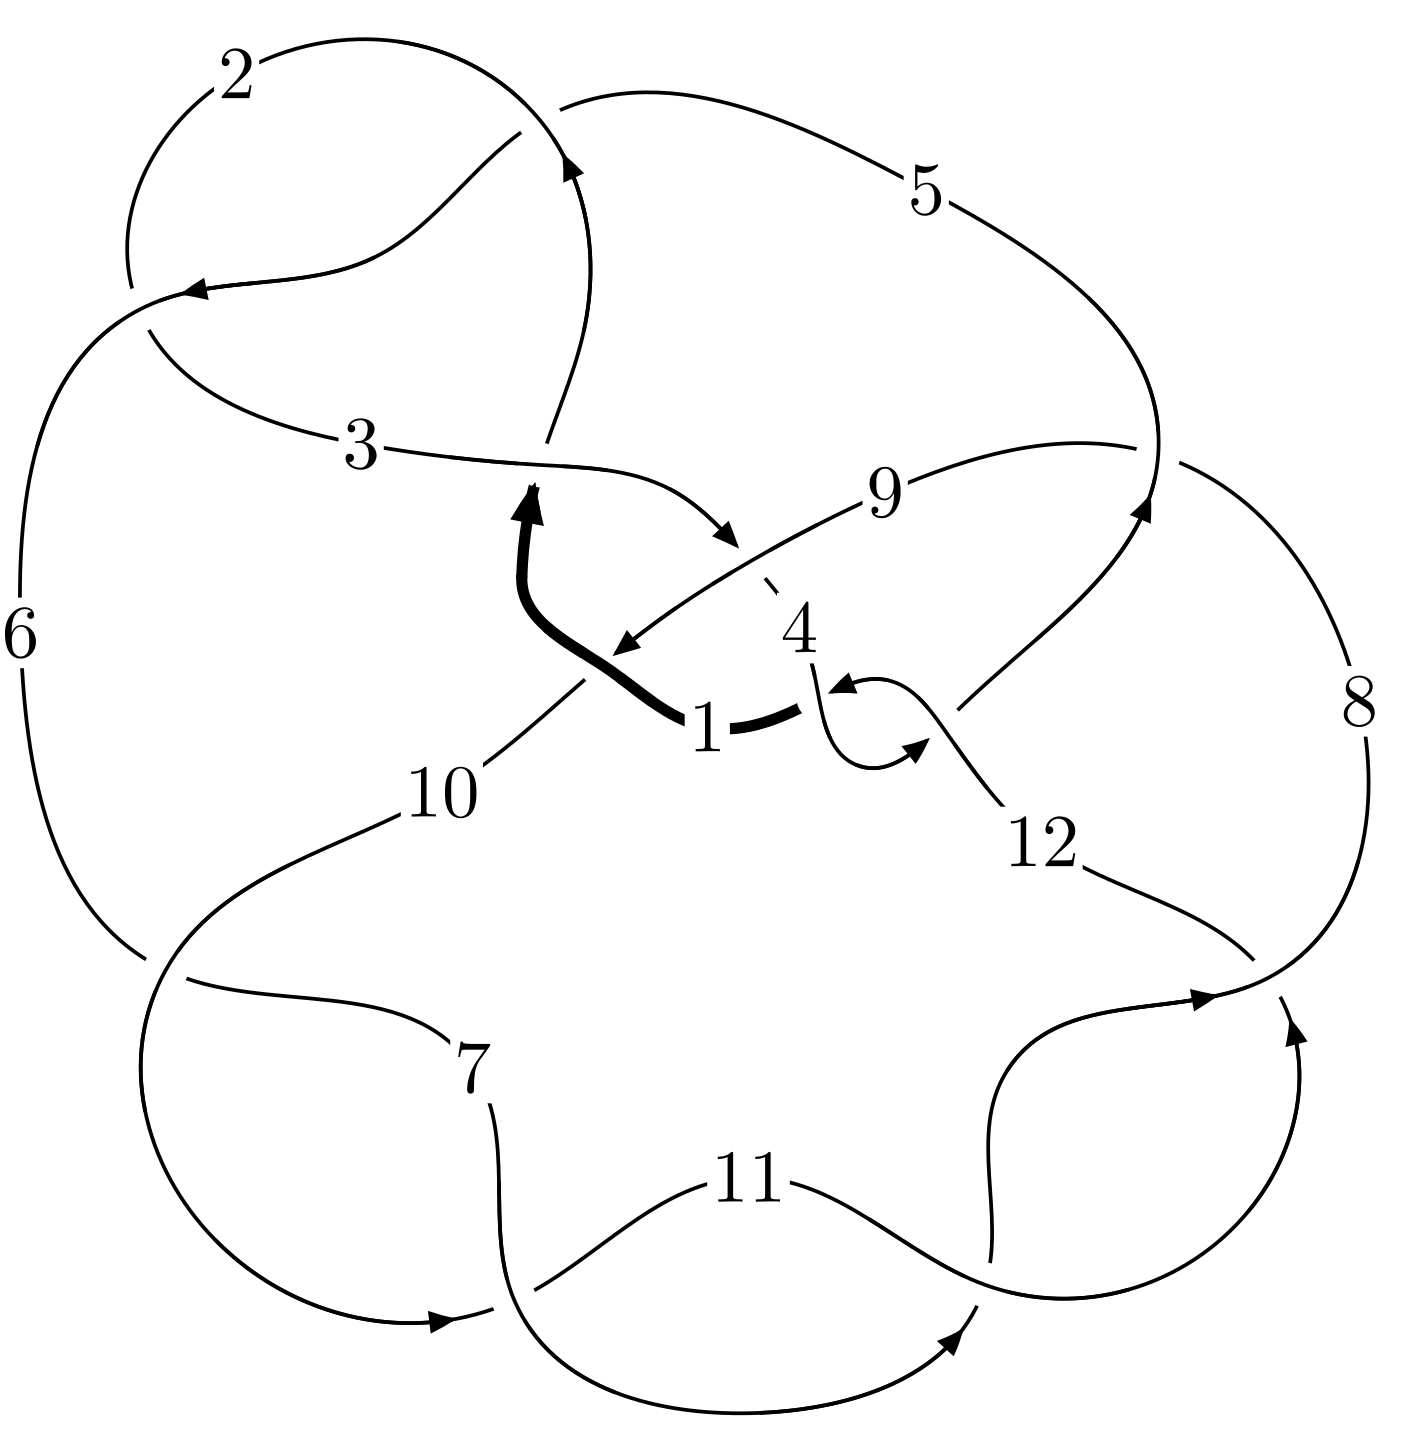
\includegraphics[width=112pt]{../../../GIT/diagram.site/Diagrams/png/1210_12a_0409.png}\\
\ \ \ A knot diagram\footnotemark}&
\allowdisplaybreaks
\textbf{Linearized knot diagam} \\
\cline{2-2}
 &
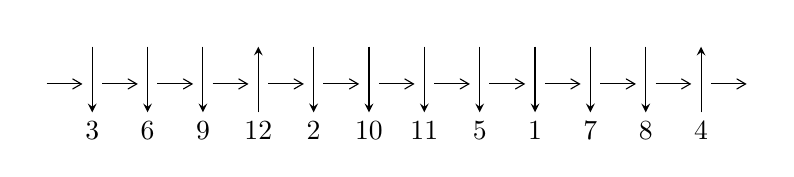
\begin{tikzpicture}[x=20pt, y=17pt]
	% nodes
	\node (C0) at (0, 0) {};
	\node (C1) at (1, 0) {};
	\node (C1U) at (1, +1) {};
	\node (C1D) at (1, -1) {3};

	\node (C2) at (2, 0) {};
	\node (C2U) at (2, +1) {};
	\node (C2D) at (2, -1) {6};

	\node (C3) at (3, 0) {};
	\node (C3U) at (3, +1) {};
	\node (C3D) at (3, -1) {9};

	\node (C4) at (4, 0) {};
	\node (C4U) at (4, +1) {};
	\node (C4D) at (4, -1) {12};

	\node (C5) at (5, 0) {};
	\node (C5U) at (5, +1) {};
	\node (C5D) at (5, -1) {2};

	\node (C6) at (6, 0) {};
	\node (C6U) at (6, +1) {};
	\node (C6D) at (6, -1) {10};

	\node (C7) at (7, 0) {};
	\node (C7U) at (7, +1) {};
	\node (C7D) at (7, -1) {11};

	\node (C8) at (8, 0) {};
	\node (C8U) at (8, +1) {};
	\node (C8D) at (8, -1) {5};

	\node (C9) at (9, 0) {};
	\node (C9U) at (9, +1) {};
	\node (C9D) at (9, -1) {1};

	\node (C10) at (10, 0) {};
	\node (C10U) at (10, +1) {};
	\node (C10D) at (10, -1) {7};

	\node (C11) at (11, 0) {};
	\node (C11U) at (11, +1) {};
	\node (C11D) at (11, -1) {8};

	\node (C12) at (12, 0) {};
	\node (C12U) at (12, +1) {};
	\node (C12D) at (12, -1) {4};
	\node (C13) at (13, 0) {};

	% arrows
	\draw[->,>={angle 60}]
	(C0) edge (C1) (C1) edge (C2) (C2) edge (C3) (C3) edge (C4) (C4) edge (C5) (C5) edge (C6) (C6) edge (C7) (C7) edge (C8) (C8) edge (C9) (C9) edge (C10) (C10) edge (C11) (C11) edge (C12) (C12) edge (C13) ;	\draw[->,>=stealth]
	(C1U) edge (C1D) (C2U) edge (C2D) (C3U) edge (C3D) (C4D) edge (C4U) (C5U) edge (C5D) (C6U) edge (C6D) (C7U) edge (C7D) (C8U) edge (C8D) (C9U) edge (C9D) (C10U) edge (C10D) (C11U) edge (C11D) (C12D) edge (C12U) ;
	\end{tikzpicture} \\
\hhline{~~} \\& 
\textbf{Solving Sequence} \\ \cline{2-2} 
 &
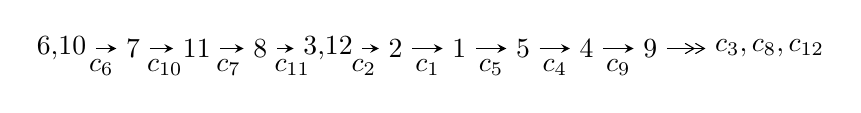
\begin{tikzpicture}[x=23pt, y=7pt]
	% node
	\node (A0) at (-1/8, 0) {6,10};
	\node (A1) at (1, 0) {7};
	\node (A2) at (2, 0) {11};
	\node (A3) at (3, 0) {8};
	\node (A4) at (65/16, 0) {3,12};
	\node (A5) at (41/8, 0) {2};
	\node (A6) at (49/8, 0) {1};
	\node (A7) at (57/8, 0) {5};
	\node (A8) at (65/8, 0) {4};
	\node (A9) at (73/8, 0) {9};
	\node (C1) at (1/2, -1) {$c_{6}$};
	\node (C2) at (3/2, -1) {$c_{10}$};
	\node (C3) at (5/2, -1) {$c_{7}$};
	\node (C4) at (7/2, -1) {$c_{11}$};
	\node (C5) at (37/8, -1) {$c_{2}$};
	\node (C6) at (45/8, -1) {$c_{1}$};
	\node (C7) at (53/8, -1) {$c_{5}$};
	\node (C8) at (61/8, -1) {$c_{4}$};
	\node (C9) at (69/8, -1) {$c_{9}$};
	\node (A10) at (11, 0) {$c_{3},c_{8},c_{12}$};

	% edge
	\draw[->,>=stealth]	
	(A0) edge (A1) (A1) edge (A2) (A2) edge (A3) (A3) edge (A4) (A4) edge (A5) (A5) edge (A6) (A6) edge (A7) (A7) edge (A8) (A8) edge (A9) ;
	\draw[->>,>={angle 60}]	
	(A9) edge (A10);
\end{tikzpicture} \\ 

\end{tabular} \\

\footnotetext{
The image of knot diagram is generated by the software ``\textbf{Draw programme}" developed by Andrew Bartholomew(\url{http://www.layer8.co.uk/maths/draw/index.htm\#Running-draw}), where we modified some parts for our purpose(\url{https://github.com/CATsTAILs/LinksPainter}).
}\phantom \\ \newline 
\centering \textbf{Ideals for irreducible components\footnotemark of $X_{\text{par}}$} 
 
\begin{align*}
I^u_{1}&=\langle 
1.36563\times10^{102} u^{76}-6.07669\times10^{102} u^{75}+\cdots+1.56636\times10^{101} b-2.53112\times10^{102},\\
\phantom{I^u_{1}}&\phantom{= \langle  }1.74520\times10^{103} u^{76}-7.65702\times10^{103} u^{75}+\cdots+7.83180\times10^{100} a-2.71806\times10^{103},\;u^{77}-5 u^{76}+\cdots-21 u+1\rangle \\
I^u_{2}&=\langle 
- a^2+2 b,\;a^4-2 a^3+2 a^2-4 a+4,\;u-1\rangle \\
\\
\end{align*}
\raggedright * 2 irreducible components of $\dim_{\mathbb{C}}=0$, with total 81 representations.\\
\footnotetext{All coefficients of polynomials are rational numbers. But the coefficients are sometimes approximated in decimal forms when there is not enough margin.}
\newpage
\renewcommand{\arraystretch}{1}
\centering \section*{I. $I^u_{1}= \langle 1.37\times10^{102} u^{76}-6.08\times10^{102} u^{75}+\cdots+1.57\times10^{101} b-2.53\times10^{102},\;1.75\times10^{103} u^{76}-7.66\times10^{103} u^{75}+\cdots+7.83\times10^{100} a-2.72\times10^{103},\;u^{77}-5 u^{76}+\cdots-21 u+1 \rangle$}
\flushleft \textbf{(i) Arc colorings}\\
\begin{tabular}{m{7pt} m{180pt} m{7pt} m{180pt} }
\flushright $a_{6}=$&$\begin{pmatrix}1\\0\end{pmatrix}$ \\
\flushright $a_{10}=$&$\begin{pmatrix}0\\u\end{pmatrix}$ \\
\flushright $a_{7}=$&$\begin{pmatrix}1\\u^2\end{pmatrix}$ \\
\flushright $a_{11}=$&$\begin{pmatrix}- u\\- u^3+u\end{pmatrix}$ \\
\flushright $a_{8}=$&$\begin{pmatrix}- u^2+1\\- u^4+2 u^2\end{pmatrix}$ \\
\flushright $a_{3}=$&$\begin{pmatrix}-222.835 u^{76}+977.683 u^{75}+\cdots-6806.53 u+347.055\\-8.71850 u^{76}+38.7950 u^{75}+\cdots-311.143 u+16.1592\end{pmatrix}$ \\
\flushright $a_{12}=$&$\begin{pmatrix}u^3-2 u\\u^5-3 u^3+u\end{pmatrix}$ \\
\flushright $a_{2}=$&$\begin{pmatrix}-231.553 u^{76}+1016.48 u^{75}+\cdots-7117.67 u+363.214\\-8.71850 u^{76}+38.7950 u^{75}+\cdots-311.143 u+16.1592\end{pmatrix}$ \\
\flushright $a_{1}=$&$\begin{pmatrix}-347.436 u^{76}+1528.95 u^{75}+\cdots-11419.1 u+612.993\\8.56092 u^{76}-38.6252 u^{75}+\cdots+321.987 u-18.8227\end{pmatrix}$ \\
\flushright $a_{5}=$&$\begin{pmatrix}86.7977 u^{76}-385.491 u^{75}+\cdots+3342.73 u-188.896\\15.5783 u^{76}-67.5759 u^{75}+\cdots+440.398 u-21.5051\end{pmatrix}$ \\
\flushright $a_{4}=$&$\begin{pmatrix}67.6379 u^{76}-301.817 u^{75}+\cdots+2732.19 u-156.914\\16.0006 u^{76}-69.5975 u^{75}+\cdots+461.286 u-22.7965\end{pmatrix}$ \\
\flushright $a_{9}=$&$\begin{pmatrix}-1492.68 u^{76}+6577.28 u^{75}+\cdots-48928.0 u+2566.44\\-157.740 u^{76}+692.289 u^{75}+\cdots-4990.09 u+254.857\end{pmatrix}$\\&\end{tabular}
\flushleft \textbf{(ii) Obstruction class $= -1$}\\~\\
\flushleft \textbf{(iii) Cusp Shapes $= 213.329 u^{76}-938.680 u^{75}+\cdots+6844.56 u-366.282$}\\~\\
\newpage\renewcommand{\arraystretch}{1}
\flushleft \textbf{(iv) u-Polynomials at the component}\newline \\
\begin{tabular}{m{50pt}|m{274pt}}
Crossings & \hspace{64pt}u-Polynomials at each crossing \\
\hline $$\begin{aligned}c_{1}\end{aligned}$$&$\begin{aligned}
&u^{77}+35 u^{76}+\cdots+129 u+4
\end{aligned}$\\
\hline $$\begin{aligned}c_{2},c_{5}\end{aligned}$$&$\begin{aligned}
&u^{77}+5 u^{76}+\cdots+23 u+2
\end{aligned}$\\
\hline $$\begin{aligned}c_{3}\end{aligned}$$&$\begin{aligned}
&u^{77}- u^{76}+\cdots+11 u-1
\end{aligned}$\\
\hline $$\begin{aligned}c_{4},c_{12}\end{aligned}$$&$\begin{aligned}
&u^{77}+5 u^{76}+\cdots+13 u+1
\end{aligned}$\\
\hline $$\begin{aligned}c_{6},c_{7},c_{10}\\c_{11}\end{aligned}$$&$\begin{aligned}
&u^{77}+5 u^{76}+\cdots-21 u-1
\end{aligned}$\\
\hline $$\begin{aligned}c_{8}\end{aligned}$$&$\begin{aligned}
&u^{77}+19 u^{76}+\cdots-1017075 u-2694247
\end{aligned}$\\
\hline $$\begin{aligned}c_{9}\end{aligned}$$&$\begin{aligned}
&u^{77}+11 u^{76}+\cdots-34199 u-5203
\end{aligned}$\\
\hline
\end{tabular}\\~\\
\newpage\renewcommand{\arraystretch}{1}
\flushleft \textbf{(v) Riley Polynomials at the component}\newline \\
\begin{tabular}{m{50pt}|m{274pt}}
Crossings & \hspace{64pt}Riley Polynomials at each crossing \\
\hline $$\begin{aligned}c_{1}\end{aligned}$$&$\begin{aligned}
&y^{77}+17 y^{76}+\cdots+16241 y-16
\end{aligned}$\\
\hline $$\begin{aligned}c_{2},c_{5}\end{aligned}$$&$\begin{aligned}
&y^{77}-35 y^{76}+\cdots+129 y-4
\end{aligned}$\\
\hline $$\begin{aligned}c_{3}\end{aligned}$$&$\begin{aligned}
&y^{77}- y^{76}+\cdots+113 y-1
\end{aligned}$\\
\hline $$\begin{aligned}c_{4},c_{12}\end{aligned}$$&$\begin{aligned}
&y^{77}+63 y^{76}+\cdots+y-1
\end{aligned}$\\
\hline $$\begin{aligned}c_{6},c_{7},c_{10}\\c_{11}\end{aligned}$$&$\begin{aligned}
&y^{77}-93 y^{76}+\cdots+161 y-1
\end{aligned}$\\
\hline $$\begin{aligned}c_{8}\end{aligned}$$&$\begin{aligned}
&y^{77}-315 y^{76}+\cdots+223681910731807 y-7258966897009
\end{aligned}$\\
\hline $$\begin{aligned}c_{9}\end{aligned}$$&$\begin{aligned}
&y^{77}+241 y^{76}+\cdots+1048539415 y-27071209
\end{aligned}$\\
\hline
\end{tabular}\\~\\
\newpage\flushleft \textbf{(vi) Complex Volumes and Cusp Shapes}
$$\begin{array}{c|c|c}  
\text{Solutions to }I^u_{1}& \I (\text{vol} + \sqrt{-1}CS) & \text{Cusp shape}\\
 \hline 
\begin{aligned}
u &= -0.871635 + 0.521957 I \\
a &= \phantom{-}0.806284 + 0.772806 I \\
b &= -0.423802 - 0.855380 I\end{aligned}
 & -3.37937 + 7.74744 I & \phantom{-0.000000 } 0 \\ \hline\begin{aligned}
u &= -0.871635 - 0.521957 I \\
a &= \phantom{-}0.806284 - 0.772806 I \\
b &= -0.423802 + 0.855380 I\end{aligned}
 & -3.37937 - 7.74744 I & \phantom{-0.000000 } 0 \\ \hline\begin{aligned}
u &= \phantom{-}0.849846 + 0.434640 I \\
a &= -0.359051 + 1.128330 I \\
b &= -0.074629 - 0.367441 I\end{aligned}
 & -3.72246 - 0.44807 I & \phantom{-0.000000 } 0 \\ \hline\begin{aligned}
u &= \phantom{-}0.849846 - 0.434640 I \\
a &= -0.359051 - 1.128330 I \\
b &= -0.074629 + 0.367441 I\end{aligned}
 & -3.72246 + 0.44807 I & \phantom{-0.000000 } 0 \\ \hline\begin{aligned}
u &= -1.008120 + 0.363672 I \\
a &= \phantom{-}0.329054 + 0.212618 I \\
b &= \phantom{-}1.196760 + 0.069492 I\end{aligned}
 & -9.11045 + 5.28746 I & \phantom{-0.000000 } 0 \\ \hline\begin{aligned}
u &= -1.008120 - 0.363672 I \\
a &= \phantom{-}0.329054 - 0.212618 I \\
b &= \phantom{-}1.196760 - 0.069492 I\end{aligned}
 & -9.11045 - 5.28746 I & \phantom{-0.000000 } 0 \\ \hline\begin{aligned}
u &= \phantom{-}0.788462 + 0.754022 I \\
a &= -0.04992 - 1.69456 I \\
b &= \phantom{-}1.045250 + 0.397646 I\end{aligned}
 & -6.31504 - 3.48175 I & \phantom{-0.000000 } 0 \\ \hline\begin{aligned}
u &= \phantom{-}0.788462 - 0.754022 I \\
a &= -0.04992 + 1.69456 I \\
b &= \phantom{-}1.045250 - 0.397646 I\end{aligned}
 & -6.31504 + 3.48175 I & \phantom{-0.000000 } 0 \\ \hline\begin{aligned}
u &= \phantom{-}0.889138 + 0.185542 I \\
a &= \phantom{-}0.481935 - 0.278927 I \\
b &= \phantom{-}0.910187 - 0.481008 I\end{aligned}
 & -1.73035 + 1.95114 I & \phantom{-0.000000 } 0 \\ \hline\begin{aligned}
u &= \phantom{-}0.889138 - 0.185542 I \\
a &= \phantom{-}0.481935 + 0.278927 I \\
b &= \phantom{-}0.910187 + 0.481008 I\end{aligned}
 & -1.73035 - 1.95114 I & \phantom{-0.000000 } 0\\
 \hline 
 \end{array}$$\newpage$$\begin{array}{c|c|c}  
\text{Solutions to }I^u_{1}& \I (\text{vol} + \sqrt{-1}CS) & \text{Cusp shape}\\
 \hline 
\begin{aligned}
u &= -0.924156 + 0.594199 I \\
a &= -0.33784 - 1.89395 I \\
b &= -1.124630 + 0.628045 I\end{aligned}
 & -5.4921 + 13.2430 I & \phantom{-0.000000 } 0 \\ \hline\begin{aligned}
u &= -0.924156 - 0.594199 I \\
a &= -0.33784 + 1.89395 I \\
b &= -1.124630 - 0.628045 I\end{aligned}
 & -5.4921 - 13.2430 I & \phantom{-0.000000 } 0 \\ \hline\begin{aligned}
u &= -0.788058 + 0.431200 I \\
a &= \phantom{-}0.57941 + 1.85354 I \\
b &= \phantom{-}1.125230 - 0.619677 I\end{aligned}
 & -0.72268 + 8.28581 I & \phantom{-0.000000 } 0 \\ \hline\begin{aligned}
u &= -0.788058 - 0.431200 I \\
a &= \phantom{-}0.57941 - 1.85354 I \\
b &= \phantom{-}1.125230 + 0.619677 I\end{aligned}
 & -0.72268 - 8.28581 I & \phantom{-0.000000 } 0 \\ \hline\begin{aligned}
u &= -0.003925 + 0.882924 I \\
a &= \phantom{-}0.80702 + 1.44156 I \\
b &= -1.073580 - 0.572372 I\end{aligned}
 & -2.67980 - 8.37636 I & \phantom{-0.000000 } 0 \\ \hline\begin{aligned}
u &= -0.003925 - 0.882924 I \\
a &= \phantom{-}0.80702 - 1.44156 I \\
b &= -1.073580 + 0.572372 I\end{aligned}
 & -2.67980 + 8.37636 I & \phantom{-0.000000 } 0 \\ \hline\begin{aligned}
u &= \phantom{-}0.297530 + 0.762269 I \\
a &= -0.783831 + 0.708395 I \\
b &= \phantom{-}1.009260 - 0.219949 I\end{aligned}
 & -4.99404 - 1.67489 I & \phantom{-0.000000 } 0 \\ \hline\begin{aligned}
u &= \phantom{-}0.297530 - 0.762269 I \\
a &= -0.783831 - 0.708395 I \\
b &= \phantom{-}1.009260 + 0.219949 I\end{aligned}
 & -4.99404 + 1.67489 I & \phantom{-0.000000 } 0 \\ \hline\begin{aligned}
u &= -0.817383\phantom{ +0.000000I} \\
a &= -0.614795\phantom{ +0.000000I} \\
b &= -1.27028\phantom{ +0.000000I}\end{aligned}
 & -4.46353\phantom{ +0.000000I} & \phantom{-0.000000 } 0 \\ \hline\begin{aligned}
u &= \phantom{-}1.143130 + 0.308998 I \\
a &= -0.393897 + 1.339210 I \\
b &= -0.667233 - 0.206047 I\end{aligned}
 & -4.00145 - 0.28027 I & \phantom{-0.000000 } 0\\
 \hline 
 \end{array}$$\newpage$$\begin{array}{c|c|c}  
\text{Solutions to }I^u_{1}& \I (\text{vol} + \sqrt{-1}CS) & \text{Cusp shape}\\
 \hline 
\begin{aligned}
u &= \phantom{-}1.143130 - 0.308998 I \\
a &= -0.393897 - 1.339210 I \\
b &= -0.667233 + 0.206047 I\end{aligned}
 & -4.00145 + 0.28027 I & \phantom{-0.000000 } 0 \\ \hline\begin{aligned}
u &= \phantom{-}1.226660 + 0.068946 I \\
a &= \phantom{-}0.424240 - 0.795406 I \\
b &= \phantom{-}0.793103 + 0.587761 I\end{aligned}
 & -1.57293 - 2.28596 I & \phantom{-0.000000 } 0 \\ \hline\begin{aligned}
u &= \phantom{-}1.226660 - 0.068946 I \\
a &= \phantom{-}0.424240 + 0.795406 I \\
b &= \phantom{-}0.793103 - 0.587761 I\end{aligned}
 & -1.57293 + 2.28596 I & \phantom{-0.000000 } 0 \\ \hline\begin{aligned}
u &= -0.765979 + 0.060037 I \\
a &= -0.505222 - 1.217440 I \\
b &= -1.165500 + 0.677513 I\end{aligned}
 & -4.10595 + 2.48021 I & \phantom{-0.000000 } 0 \\ \hline\begin{aligned}
u &= -0.765979 - 0.060037 I \\
a &= -0.505222 + 1.217440 I \\
b &= -1.165500 - 0.677513 I\end{aligned}
 & -4.10595 - 2.48021 I & \phantom{-0.000000 } 0 \\ \hline\begin{aligned}
u &= \phantom{-}1.065830 + 0.645154 I \\
a &= \phantom{-}0.282851 - 0.390245 I \\
b &= -1.048050 + 0.473536 I\end{aligned}
 & -5.82204 + 3.18193 I & \phantom{-0.000000 } 0 \\ \hline\begin{aligned}
u &= \phantom{-}1.065830 - 0.645154 I \\
a &= \phantom{-}0.282851 + 0.390245 I \\
b &= -1.048050 - 0.473536 I\end{aligned}
 & -5.82204 - 3.18193 I & \phantom{-0.000000 } 0 \\ \hline\begin{aligned}
u &= -0.654081 + 0.366173 I \\
a &= -0.800157 - 0.489010 I \\
b &= \phantom{-}0.384980 + 0.843441 I\end{aligned}
 & \phantom{-}1.46897 + 2.86772 I & \phantom{-0.000000 } 0 \\ \hline\begin{aligned}
u &= -0.654081 - 0.366173 I \\
a &= -0.800157 + 0.489010 I \\
b &= \phantom{-}0.384980 - 0.843441 I\end{aligned}
 & \phantom{-}1.46897 - 2.86772 I & \phantom{-0.000000 } 0 \\ \hline\begin{aligned}
u &= -0.028223 + 0.746166 I \\
a &= \phantom{-}0.40028 - 1.68284 I \\
b &= -0.431130 + 0.682340 I\end{aligned}
 & -0.80801 - 3.51202 I & -8.00000 + 0. I\phantom{ +0.000000I}\\
 \hline 
 \end{array}$$\newpage$$\begin{array}{c|c|c}  
\text{Solutions to }I^u_{1}& \I (\text{vol} + \sqrt{-1}CS) & \text{Cusp shape}\\
 \hline 
\begin{aligned}
u &= -0.028223 - 0.746166 I \\
a &= \phantom{-}0.40028 + 1.68284 I \\
b &= -0.431130 - 0.682340 I\end{aligned}
 & -0.80801 + 3.51202 I & -8.00000 + 0. I\phantom{ +0.000000I} \\ \hline\begin{aligned}
u &= -0.701002 + 0.185836 I \\
a &= \phantom{-}0.127831 - 0.967471 I \\
b &= -0.614469 + 0.908672 I\end{aligned}
 & -2.32786 + 3.73049 I & -13.7491 - 12.8450 I \\ \hline\begin{aligned}
u &= -0.701002 - 0.185836 I \\
a &= \phantom{-}0.127831 + 0.967471 I \\
b &= -0.614469 - 0.908672 I\end{aligned}
 & -2.32786 - 3.73049 I & -13.7491 + 12.8450 I \\ \hline\begin{aligned}
u &= \phantom{-}0.618969 + 0.344051 I \\
a &= -0.51111 + 2.87161 I \\
b &= -0.944612 - 0.463574 I\end{aligned}
 & -1.67002 - 3.05655 I & -8.00000 + 6.69690 I \\ \hline\begin{aligned}
u &= \phantom{-}0.618969 - 0.344051 I \\
a &= -0.51111 - 2.87161 I \\
b &= -0.944612 + 0.463574 I\end{aligned}
 & -1.67002 + 3.05655 I & -8.00000 - 6.69690 I \\ \hline\begin{aligned}
u &= -0.083013 + 0.598652 I \\
a &= -1.12653 - 1.23667 I \\
b &= \phantom{-}1.022510 + 0.594189 I\end{aligned}
 & \phantom{-}1.39951 - 4.78176 I & -4.95226 + 4.64563 I \\ \hline\begin{aligned}
u &= -0.083013 - 0.598652 I \\
a &= -1.12653 + 1.23667 I \\
b &= \phantom{-}1.022510 - 0.594189 I\end{aligned}
 & \phantom{-}1.39951 + 4.78176 I & -4.95226 - 4.64563 I \\ \hline\begin{aligned}
u &= \phantom{-}0.601180 + 0.002263 I \\
a &= -14.1881 + 11.7877 I \\
b &= \phantom{-}0.851370 + 0.493083 I\end{aligned}
 & -2.60411 - 2.03169 I & -136.2940 - 14.6490 I \\ \hline\begin{aligned}
u &= \phantom{-}0.601180 - 0.002263 I \\
a &= -14.1881 - 11.7877 I \\
b &= \phantom{-}0.851370 - 0.493083 I\end{aligned}
 & -2.60411 + 2.03169 I & -136.2940 + 14.6490 I \\ \hline\begin{aligned}
u &= -0.212039 + 0.506396 I \\
a &= -0.10650 + 1.80456 I \\
b &= \phantom{-}0.564116 - 0.692422 I\end{aligned}
 & \phantom{-}2.77376 + 0.18726 I & -1.78780 - 2.14448 I\\
 \hline 
 \end{array}$$\newpage$$\begin{array}{c|c|c}  
\text{Solutions to }I^u_{1}& \I (\text{vol} + \sqrt{-1}CS) & \text{Cusp shape}\\
 \hline 
\begin{aligned}
u &= -0.212039 - 0.506396 I \\
a &= -0.10650 - 1.80456 I \\
b &= \phantom{-}0.564116 + 0.692422 I\end{aligned}
 & \phantom{-}2.77376 - 0.18726 I & -1.78780 + 2.14448 I \\ \hline\begin{aligned}
u &= \phantom{-}0.348984 + 0.348224 I \\
a &= \phantom{-}1.94963 - 0.62772 I \\
b &= -0.814043 + 0.325199 I\end{aligned}
 & -0.965555 + 0.405754 I & -7.83651 + 1.83330 I \\ \hline\begin{aligned}
u &= \phantom{-}0.348984 - 0.348224 I \\
a &= \phantom{-}1.94963 + 0.62772 I \\
b &= -0.814043 - 0.325199 I\end{aligned}
 & -0.965555 - 0.405754 I & -7.83651 - 1.83330 I \\ \hline\begin{aligned}
u &= \phantom{-}0.479840\phantom{ +0.000000I} \\
a &= \phantom{-}0.890816\phantom{ +0.000000I} \\
b &= -0.179116\phantom{ +0.000000I}\end{aligned}
 & -0.737088\phantom{ +0.000000I} & -13.2280\phantom{ +0.000000I} \\ \hline\begin{aligned}
u &= -1.57486 + 0.04270 I \\
a &= \phantom{-}0.597648 + 0.370331 I \\
b &= -0.420518 - 0.504083 I\end{aligned}
 & -7.73145 + 0.41162 I & \phantom{-0.000000 } 0 \\ \hline\begin{aligned}
u &= -1.57486 - 0.04270 I \\
a &= \phantom{-}0.597648 - 0.370331 I \\
b &= -0.420518 + 0.504083 I\end{aligned}
 & -7.73145 - 0.41162 I & \phantom{-0.000000 } 0 \\ \hline\begin{aligned}
u &= -1.60958 + 0.01197 I \\
a &= -2.62680 - 0.11024 I \\
b &= \phantom{-}0.753976 - 0.522222 I\end{aligned}
 & -10.36160 + 2.12144 I & \phantom{-0.000000 } 0 \\ \hline\begin{aligned}
u &= -1.60958 - 0.01197 I \\
a &= -2.62680 + 0.11024 I \\
b &= \phantom{-}0.753976 + 0.522222 I\end{aligned}
 & -10.36160 - 2.12144 I & \phantom{-0.000000 } 0 \\ \hline\begin{aligned}
u &= \phantom{-}1.61089 + 0.07581 I \\
a &= -0.267958 + 0.344213 I \\
b &= \phantom{-}0.304142 - 1.035400 I\end{aligned}
 & -6.33159 - 4.36200 I & \phantom{-0.000000 } 0 \\ \hline\begin{aligned}
u &= \phantom{-}1.61089 - 0.07581 I \\
a &= -0.267958 - 0.344213 I \\
b &= \phantom{-}0.304142 + 1.035400 I\end{aligned}
 & -6.33159 + 4.36200 I & \phantom{-0.000000 } 0\\
 \hline 
 \end{array}$$\newpage$$\begin{array}{c|c|c}  
\text{Solutions to }I^u_{1}& \I (\text{vol} + \sqrt{-1}CS) & \text{Cusp shape}\\
 \hline 
\begin{aligned}
u &= -1.61710 + 0.08976 I \\
a &= -1.02416 - 1.56228 I \\
b &= -1.037440 + 0.506606 I\end{aligned}
 & -9.47283 + 4.60615 I & \phantom{-0.000000 } 0 \\ \hline\begin{aligned}
u &= -1.61710 - 0.08976 I \\
a &= -1.02416 + 1.56228 I \\
b &= -1.037440 - 0.506606 I\end{aligned}
 & -9.47283 - 4.60615 I & \phantom{-0.000000 } 0 \\ \hline\begin{aligned}
u &= \phantom{-}1.63407 + 0.03802 I \\
a &= \phantom{-}0.003139 + 0.666872 I \\
b &= -0.669565 - 1.103280 I\end{aligned}
 & -10.52050 - 4.48505 I & \phantom{-0.000000 } 0 \\ \hline\begin{aligned}
u &= \phantom{-}1.63407 - 0.03802 I \\
a &= \phantom{-}0.003139 - 0.666872 I \\
b &= -0.669565 + 1.103280 I\end{aligned}
 & -10.52050 + 4.48505 I & \phantom{-0.000000 } 0 \\ \hline\begin{aligned}
u &= -1.64816 + 0.01239 I \\
a &= \phantom{-}1.51628 + 0.07749 I \\
b &= \phantom{-}0.960623 + 0.388315 I\end{aligned}
 & -10.42720 - 1.45912 I & \phantom{-0.000000 } 0 \\ \hline\begin{aligned}
u &= -1.64816 - 0.01239 I \\
a &= \phantom{-}1.51628 - 0.07749 I \\
b &= \phantom{-}0.960623 - 0.388315 I\end{aligned}
 & -10.42720 + 1.45912 I & \phantom{-0.000000 } 0 \\ \hline\begin{aligned}
u &= \phantom{-}1.64827 + 0.01455 I \\
a &= -0.559053 + 0.775844 I \\
b &= -1.30014 - 0.75889 I\end{aligned}
 & -12.59660 - 2.75325 I & \phantom{-0.000000 } 0 \\ \hline\begin{aligned}
u &= \phantom{-}1.64827 - 0.01455 I \\
a &= -0.559053 - 0.775844 I \\
b &= -1.30014 + 0.75889 I\end{aligned}
 & -12.59660 + 2.75325 I & \phantom{-0.000000 } 0 \\ \hline\begin{aligned}
u &= \phantom{-}1.64464 + 0.11365 I \\
a &= \phantom{-}0.85856 - 1.15813 I \\
b &= \phantom{-}1.210340 + 0.641926 I\end{aligned}
 & -9.11064 - 10.32360 I & \phantom{-0.000000 } 0 \\ \hline\begin{aligned}
u &= \phantom{-}1.64464 - 0.11365 I \\
a &= \phantom{-}0.85856 + 1.15813 I \\
b &= \phantom{-}1.210340 - 0.641926 I\end{aligned}
 & -9.11064 + 10.32360 I & \phantom{-0.000000 } 0\\
 \hline 
 \end{array}$$\newpage$$\begin{array}{c|c|c}  
\text{Solutions to }I^u_{1}& \I (\text{vol} + \sqrt{-1}CS) & \text{Cusp shape}\\
 \hline 
\begin{aligned}
u &= -0.095003 + 0.332687 I \\
a &= \phantom{-}2.10515 - 0.52416 I \\
b &= -0.435064 - 0.531419 I\end{aligned}
 & -0.66814 - 1.87825 I & -4.74322 + 2.54988 I \\ \hline\begin{aligned}
u &= -0.095003 - 0.332687 I \\
a &= \phantom{-}2.10515 + 0.52416 I \\
b &= -0.435064 + 0.531419 I\end{aligned}
 & -0.66814 + 1.87825 I & -4.74322 - 2.54988 I \\ \hline\begin{aligned}
u &= \phantom{-}1.65568\phantom{ +0.000000I} \\
a &= -0.782927\phantom{ +0.000000I} \\
b &= -1.47869\phantom{ +0.000000I}\end{aligned}
 & -13.1360\phantom{ +0.000000I} & \phantom{-0.000000 } 0 \\ \hline\begin{aligned}
u &= -1.65750 + 0.14801 I \\
a &= -0.335612 - 0.692340 I \\
b &= \phantom{-}0.230603 + 0.666767 I\end{aligned}
 & -12.26620 + 2.82177 I & \phantom{-0.000000 } 0 \\ \hline\begin{aligned}
u &= -1.65750 - 0.14801 I \\
a &= -0.335612 + 0.692340 I \\
b &= \phantom{-}0.230603 - 0.666767 I\end{aligned}
 & -12.26620 - 2.82177 I & \phantom{-0.000000 } 0 \\ \hline\begin{aligned}
u &= \phantom{-}1.67002 + 0.14858 I \\
a &= \phantom{-}0.473642 - 0.470437 I \\
b &= -0.414424 + 0.964985 I\end{aligned}
 & -12.1217 - 10.3513 I & \phantom{-0.000000 } 0 \\ \hline\begin{aligned}
u &= \phantom{-}1.67002 - 0.14858 I \\
a &= \phantom{-}0.473642 + 0.470437 I \\
b &= -0.414424 - 0.964985 I\end{aligned}
 & -12.1217 + 10.3513 I & \phantom{-0.000000 } 0 \\ \hline\begin{aligned}
u &= \phantom{-}1.68810 + 0.17252 I \\
a &= -0.73378 + 1.40207 I \\
b &= -1.170620 - 0.661665 I\end{aligned}
 & -14.4500 - 16.2652 I & \phantom{-0.000000 } 0 \\ \hline\begin{aligned}
u &= \phantom{-}1.68810 - 0.17252 I \\
a &= -0.73378 - 1.40207 I \\
b &= -1.170620 + 0.661665 I\end{aligned}
 & -14.4500 + 16.2652 I & \phantom{-0.000000 } 0 \\ \hline\begin{aligned}
u &= -1.68571 + 0.22627 I \\
a &= \phantom{-}0.53610 + 1.31327 I \\
b &= \phantom{-}1.111390 - 0.508532 I\end{aligned}
 & -14.7554 + 7.3067 I & \phantom{-0.000000 } 0\\
 \hline 
 \end{array}$$\newpage$$\begin{array}{c|c|c}  
\text{Solutions to }I^u_{1}& \I (\text{vol} + \sqrt{-1}CS) & \text{Cusp shape}\\
 \hline 
\begin{aligned}
u &= -1.68571 - 0.22627 I \\
a &= \phantom{-}0.53610 - 1.31327 I \\
b &= \phantom{-}1.111390 + 0.508532 I\end{aligned}
 & -14.7554 - 7.3067 I & \phantom{-0.000000 } 0 \\ \hline\begin{aligned}
u &= \phantom{-}1.70007 + 0.09625 I \\
a &= \phantom{-}0.737615 - 0.162232 I \\
b &= \phantom{-}1.337770 - 0.063513 I\end{aligned}
 & -18.5664 - 7.1193 I & \phantom{-0.000000 } 0 \\ \hline\begin{aligned}
u &= \phantom{-}1.70007 - 0.09625 I \\
a &= \phantom{-}0.737615 + 0.162232 I \\
b &= \phantom{-}1.337770 + 0.063513 I\end{aligned}
 & -18.5664 + 7.1193 I & \phantom{-0.000000 } 0 \\ \hline\begin{aligned}
u &= -1.75832 + 0.10945 I \\
a &= -0.528353 + 0.351806 I \\
b &= -1.099490 - 0.317079 I\end{aligned}
 & -16.0277 - 0.1764 I & \phantom{-0.000000 } 0 \\ \hline\begin{aligned}
u &= -1.75832 - 0.10945 I \\
a &= -0.528353 - 0.351806 I \\
b &= -1.099490 + 0.317079 I\end{aligned}
 & -16.0277 + 0.1764 I & \phantom{-0.000000 } 0 \\ \hline\begin{aligned}
u &= \phantom{-}0.1016190 + 0.0298609 I \\
a &= \phantom{-}9.47466 + 7.93380 I \\
b &= -0.918640 - 0.537767 I\end{aligned}
 & -1.80001 - 2.05748 I & -8.74387 + 2.56472 I \\ \hline\begin{aligned}
u &= \phantom{-}0.1016190 - 0.0298609 I \\
a &= \phantom{-}9.47466 - 7.93380 I \\
b &= -0.918640 + 0.537767 I\end{aligned}
 & -1.80001 + 2.05748 I & -8.74387 - 2.56472 I\\
 \hline 
 \end{array}$$\newpage\newpage\renewcommand{\arraystretch}{1}
\centering \section*{II. $I^u_{2}= \langle - a^2+2 b,\;a^4-2 a^3+2 a^2-4 a+4,\;u-1 \rangle$}
\flushleft \textbf{(i) Arc colorings}\\
\begin{tabular}{m{7pt} m{180pt} m{7pt} m{180pt} }
\flushright $a_{6}=$&$\begin{pmatrix}1\\0\end{pmatrix}$ \\
\flushright $a_{10}=$&$\begin{pmatrix}0\\1\end{pmatrix}$ \\
\flushright $a_{7}=$&$\begin{pmatrix}1\\1\end{pmatrix}$ \\
\flushright $a_{11}=$&$\begin{pmatrix}-1\\0\end{pmatrix}$ \\
\flushright $a_{8}=$&$\begin{pmatrix}0\\1\end{pmatrix}$ \\
\flushright $a_{3}=$&$\begin{pmatrix}a\\\frac{1}{2} a^2\end{pmatrix}$ \\
\flushright $a_{12}=$&$\begin{pmatrix}-1\\-1\end{pmatrix}$ \\
\flushright $a_{2}=$&$\begin{pmatrix}\frac{1}{2} a^2+a\\\frac{1}{2} a^2\end{pmatrix}$ \\
\flushright $a_{1}=$&$\begin{pmatrix}-\frac{1}{2} a^3+\frac{1}{2} a^2+2\\-\frac{1}{2} a^3+\frac{1}{2} a^2+1\end{pmatrix}$ \\
\flushright $a_{5}=$&$\begin{pmatrix}- a^3+\frac{1}{2} a^2- a+2\\-\frac{1}{2} a^3+\frac{1}{2} a^2- a+1\end{pmatrix}$ \\
\flushright $a_{4}=$&$\begin{pmatrix}-\frac{3}{2} a^3+\frac{1}{2} a^2- a+3\\- a^3+\frac{1}{2} a^2- a+2\end{pmatrix}$ \\
\flushright $a_{9}=$&$\begin{pmatrix}-\frac{3}{2} a^3+\frac{3}{2} a^2- a+5\\- a^3+a^2- a+4\end{pmatrix}$\\&\end{tabular}
\flushleft \textbf{(ii) Obstruction class $= 1$}\\~\\
\flushleft \textbf{(iii) Cusp Shapes $= 2 a^3-2 a^2+4 a-20$}\\~\\
\newpage\renewcommand{\arraystretch}{1}
\flushleft \textbf{(iv) u-Polynomials at the component}\newline \\
\begin{tabular}{m{50pt}|m{274pt}}
Crossings & \hspace{64pt}u-Polynomials at each crossing \\
\hline $$\begin{aligned}c_{1}\end{aligned}$$&$\begin{aligned}
&(u^2- u+1)^2
\end{aligned}$\\
\hline $$\begin{aligned}c_{2},c_{5}\end{aligned}$$&$\begin{aligned}
&u^4- u^2+1
\end{aligned}$\\
\hline $$\begin{aligned}c_{3},c_{4},c_{12}\end{aligned}$$&$\begin{aligned}
&(u^2+1)^2
\end{aligned}$\\
\hline $$\begin{aligned}c_{6},c_{7}\end{aligned}$$&$\begin{aligned}
&(u-1)^4
\end{aligned}$\\
\hline $$\begin{aligned}c_{8}\end{aligned}$$&$\begin{aligned}
&u^4-2 u^3+5 u^2-4 u+1
\end{aligned}$\\
\hline $$\begin{aligned}c_{9}\end{aligned}$$&$\begin{aligned}
&u^4+4 u^3+5 u^2+2 u+1
\end{aligned}$\\
\hline $$\begin{aligned}c_{10},c_{11}\end{aligned}$$&$\begin{aligned}
&(u+1)^4
\end{aligned}$\\
\hline
\end{tabular}\\~\\
\newpage\renewcommand{\arraystretch}{1}
\flushleft \textbf{(v) Riley Polynomials at the component}\newline \\
\begin{tabular}{m{50pt}|m{274pt}}
Crossings & \hspace{64pt}Riley Polynomials at each crossing \\
\hline $$\begin{aligned}c_{1}\end{aligned}$$&$\begin{aligned}
&(y^2+y+1)^2
\end{aligned}$\\
\hline $$\begin{aligned}c_{2},c_{5}\end{aligned}$$&$\begin{aligned}
&(y^2- y+1)^2
\end{aligned}$\\
\hline $$\begin{aligned}c_{3},c_{4},c_{12}\end{aligned}$$&$\begin{aligned}
&(y+1)^4
\end{aligned}$\\
\hline $$\begin{aligned}c_{6},c_{7},c_{10}\\c_{11}\end{aligned}$$&$\begin{aligned}
&(y-1)^4
\end{aligned}$\\
\hline $$\begin{aligned}c_{8}\end{aligned}$$&$\begin{aligned}
&y^4+6 y^3+11 y^2-6 y+1
\end{aligned}$\\
\hline $$\begin{aligned}c_{9}\end{aligned}$$&$\begin{aligned}
&y^4-6 y^3+11 y^2+6 y+1
\end{aligned}$\\
\hline
\end{tabular}\\~\\
\newpage\flushleft \textbf{(vi) Complex Volumes and Cusp Shapes}
$$\begin{array}{c|c|c}  
\text{Solutions to }I^u_{2}& \I (\text{vol} + \sqrt{-1}CS) & \text{Cusp shape}\\
 \hline 
\begin{aligned}
u &= \phantom{-}1.00000\phantom{ +0.000000I} \\
a &= \phantom{-}1.36603 + 0.36603 I \\
b &= \phantom{-}0.866025 + 0.500000 I\end{aligned}
 & -3.28987 - 2.02988 I & -14.0000 + 3.4641 I \\ \hline\begin{aligned}
u &= \phantom{-}1.00000\phantom{ +0.000000I} \\
a &= \phantom{-}1.36603 - 0.36603 I \\
b &= \phantom{-}0.866025 - 0.500000 I\end{aligned}
 & -3.28987 + 2.02988 I & -14.0000 - 3.4641 I \\ \hline\begin{aligned}
u &= \phantom{-}1.00000\phantom{ +0.000000I} \\
a &= -0.36603 + 1.36603 I \\
b &= -0.866025 - 0.500000 I\end{aligned}
 & -3.28987 - 2.02988 I & -14.0000 + 3.4641 I \\ \hline\begin{aligned}
u &= \phantom{-}1.00000\phantom{ +0.000000I} \\
a &= -0.36603 - 1.36603 I \\
b &= -0.866025 + 0.500000 I\end{aligned}
 & -3.28987 + 2.02988 I & -14.0000 - 3.4641 I\\
 \hline 
 \end{array}$$\newpage
\newpage\renewcommand{\arraystretch}{1}
\centering \section*{ III. u-Polynomials}
\begin{tabular}{m{50pt}|m{274pt}}
Crossings & \hspace{64pt}u-Polynomials at each crossing \\
\hline $$\begin{aligned}c_{1}\end{aligned}$$&$\begin{aligned}
&((u^2- u+1)^2)(u^{77}+35 u^{76}+\cdots+129 u+4)
\end{aligned}$\\
\hline $$\begin{aligned}c_{2},c_{5}\end{aligned}$$&$\begin{aligned}
&(u^4- u^2+1)(u^{77}+5 u^{76}+\cdots+23 u+2)
\end{aligned}$\\
\hline $$\begin{aligned}c_{3}\end{aligned}$$&$\begin{aligned}
&((u^2+1)^2)(u^{77}- u^{76}+\cdots+11 u-1)
\end{aligned}$\\
\hline $$\begin{aligned}c_{4},c_{12}\end{aligned}$$&$\begin{aligned}
&((u^2+1)^2)(u^{77}+5 u^{76}+\cdots+13 u+1)
\end{aligned}$\\
\hline $$\begin{aligned}c_{6},c_{7}\end{aligned}$$&$\begin{aligned}
&((u-1)^4)(u^{77}+5 u^{76}+\cdots-21 u-1)
\end{aligned}$\\
\hline $$\begin{aligned}c_{8}\end{aligned}$$&$\begin{aligned}
&(u^4-2 u^3+5 u^2-4 u+1)(u^{77}+19 u^{76}+\cdots-1017075 u-2694247)
\end{aligned}$\\
\hline $$\begin{aligned}c_{9}\end{aligned}$$&$\begin{aligned}
&(u^4+4 u^3+5 u^2+2 u+1)(u^{77}+11 u^{76}+\cdots-34199 u-5203)
\end{aligned}$\\
\hline $$\begin{aligned}c_{10},c_{11}\end{aligned}$$&$\begin{aligned}
&((u+1)^4)(u^{77}+5 u^{76}+\cdots-21 u-1)
\end{aligned}$\\
\hline
\end{tabular}\newpage\renewcommand{\arraystretch}{1}
\centering \section*{ IV. Riley Polynomials}
\begin{tabular}{m{50pt}|m{274pt}}
Crossings & \hspace{64pt}Riley Polynomials at each crossing \\
\hline $$\begin{aligned}c_{1}\end{aligned}$$&$\begin{aligned}
&((y^2+y+1)^2)(y^{77}+17 y^{76}+\cdots+16241 y-16)
\end{aligned}$\\
\hline $$\begin{aligned}c_{2},c_{5}\end{aligned}$$&$\begin{aligned}
&((y^2- y+1)^2)(y^{77}-35 y^{76}+\cdots+129 y-4)
\end{aligned}$\\
\hline $$\begin{aligned}c_{3}\end{aligned}$$&$\begin{aligned}
&((y+1)^4)(y^{77}- y^{76}+\cdots+113 y-1)
\end{aligned}$\\
\hline $$\begin{aligned}c_{4},c_{12}\end{aligned}$$&$\begin{aligned}
&((y+1)^4)(y^{77}+63 y^{76}+\cdots+y-1)
\end{aligned}$\\
\hline $$\begin{aligned}c_{6},c_{7},c_{10}\\c_{11}\end{aligned}$$&$\begin{aligned}
&((y-1)^4)(y^{77}-93 y^{76}+\cdots+161 y-1)
\end{aligned}$\\
\hline $$\begin{aligned}c_{8}\end{aligned}$$&$\begin{aligned}
&(y^4+6 y^3+11 y^2-6 y+1)\\
&\cdot(y^{77}-315 y^{76}+\cdots+223681910731807 y-7258966897009)
\end{aligned}$\\
\hline $$\begin{aligned}c_{9}\end{aligned}$$&$\begin{aligned}
&(y^4-6 y^3+11 y^2+6 y+1)\\
&\cdot(y^{77}+241 y^{76}+\cdots+1048539415 y-27071209)
\end{aligned}$\\
\hline
\end{tabular}
\vskip 2pc
\end{document}